
\section{Simultaneous Localization And Mapping}
Esta sección describe los conocimientos básicos respecto a la Localización y Mapeo Simultáneos (SLAM), a la vez de introducir parte de los algoritmos y sensores conocidos.

\subsection{Introducción al SLAM}
El problema de localización y mapeo simultáneos (SLAM) se basa en el proceso de un robot que construye un mapa de su entorno desconocido (\textit{mapping}) mientras este lo explora conociendo su ubicación en el mismo (\textit{localization}). Dicho problema puede ser expresado como el dilema del huevo o la gallina, ya que para conocer la ubicación del robot es necesario determinar el mapa que lo rodea, sin embargo, para que el mismo pueda estimar el mapa en el cual se encuentra, necesita primero conocer su ubicación dentro de ese entorno. A partir de la detección y seguimiento de marcas naturales del ambiente (\textit{landmarks}), los sistemas SLAM estiman tanto la posición del robot como la ubicación de las marcas en el entorno. El mapa se construye con las estimaciones de las posiciones de dichas marcas, las cuales van siendo ajustadas a medida que son observadas desde distintas posiciones.

El SLAM es un problema difícil ya que, debido al ruido de los sensores utilizados, ninguna de las mediciones es perfecta. Esto significa que ni el movimiento del robot ni la estructura del entorno se conocen de manera absolutamente precisa, sino solo hasta cierto grado de incertidumbre. Con el fin de hacer frente a estas incertidumbres, el SLAM generalmente se entiende y se aborda mediante técnicas y modelos probabilísticos. Las diferentes formas en que se representan las funciones de densidad probabilística constituyen las diferencias en cada enfoque. Muchas de ellas utilizan filtros de Bayes, tal como lo es el Filtro de Kalman Extendido (EKF) 
\begin{large}
[DURRANT-WHYTE2006]
[KALMAN1960]
\end{large}, o en versiones más modernas, por ejemplo, el Fast-SLAM
\begin{large}
[PONER FASTSLAM BIEN]
\end{large}. 
Sin embargo, el uso de enfoques de estimación de estado para describir el problema de SLAM implica resolver una serie de inconvenientes que se generan a partir del mismo, siendo de los más destacados la \textit{asociación de datos}\textbf{[ref 103 y 104 de reid2016]} y el \textit{cierre de ciclo}.

\subsubsection{Asociación de datos}
En su forma más simple, la \textit{asociación de datos} refiere a relacionar diferentes mediciones con los objetos que se encuentran en el entorno. Si bien los sensores utilizado para este tipo de aplicaciones puede tomar miles de mediciones del entorno por segundo, generalmente no produce información suficiente para resolver estas concordancias directamente.

Con una incertidumbre siempre presente en la posición del robot, normalmente no se conoce la dirección exacta a la que apunta un sensor. Esta incertidumbre, junto con la incapacidad para identificar de qué objeto proviene cada medición, crea incertidumbres y posibles ambigüedades referidas a la distancia que se encuentra el objeto respecto al robot.

\subsubsection{Cierre de ciclo}
Cuando un robot sigue un camino largo, mientras mide su progreso con sensores incorporados, el mismo acumula incertidumbre debido al ruido inherente de los sensores. Si el robot sigue visitando nuevos lugares, la incertidumbre de la posición seguirá creciendo sin límite. Cuando el robot vuelve a visitar un lugar en el que ha estado anteriormente, se producen eventos de \textit{cierre de ciclo}
\begin{large}
[REFS DE REID Y VER CASTRO]
\end{large}, otorgando información valiosa respecto a la relación entre las estimaciones llevadas a cabo por los sistemas de localización. Tomar conocimiento de que se ha efectuado un ciclo en la trayectoria permite calcular el error cometido en la estimación de la posición y da origen a una serie de procesos que permiten corregir tanto la localización actual del robot como el mapa hasta ese momento construido.

\begin{large}
VER DE QUE MAS PONERRRRRRR
\end{large}{}

\subsection{Sensores}
Para navegar de manera robusta a través de entornos desconocidos y no estructurados, los robots deben poder percibir y modelar su entorno. Es por esto que lo que se busca es construir mapas precisos y ubicarse en los mismos utilizando solo sensores a bordo. A continuación se presentan algunos de los principales sensores para lograr lo propuesto.

\subsubsection{LiDAR}
Light Detection And Ranging, conocido como LiDAR, es una tecnología que tiene su origen en la fusión de la tecnología láser junto con la tecnología RADAR (Radio Detection And Ranging), lo cual ha permitido mejorar en gran medida la precisión de los sistemas de detección,  dando lugar a nuevas aplicaciones. 

El  fundamento de los dispositivos basados en la tecnología LIDAR es el cálculo del tiempo de vuelo (\textit{TOF -Time  Of Flight}) de los pulsos láser, de manera que, conociendo la velocidad del mismo, las características angulares con las que fue emitido, y la diferencia de tiempos entre el rayo emitido y el reflejado, se puede determinar de manera sencilla la distancia a la que se encuentra el obstáculo/objeto con el que el rayo impactó. Esto permite, con gran exactitud, conocer las coordenadas de la posición de objetos o superficies con respecto del sistema de coordenadas del propio dispositivo.

Muchos investigadores tienen sensores lidar de exploración servo-montados en configuraciones de cabeceo [116, 117] o de barrido [118] (Fig. \ref{fig:lidars}.a) para producir exploraciones tanto planares como 3D, aunque para este último caso el mismo entrega escaneos cada 1Hz o menos. Este campo de visión, sobre todo el 3D, tiene el costo de una mayor complejidad (sincronización servo temporal) y una menor cobertura en direcciones críticas.

\begin{large}
[pfingsthron2012][newman2006][bosse2009]
\end{large}

Con el fin de aumentar la frecuencia de recolección de datos, existen sensores que integran múltiples LiDAR en una sola unidad de escaneo (Fig. \ref{fig:lidars}.b), de modo que se pueden obtener escaneados en 3D completos a altas velocidades.

\begin{figure}
    \centering
    \subfloat[Scanse Sweep]{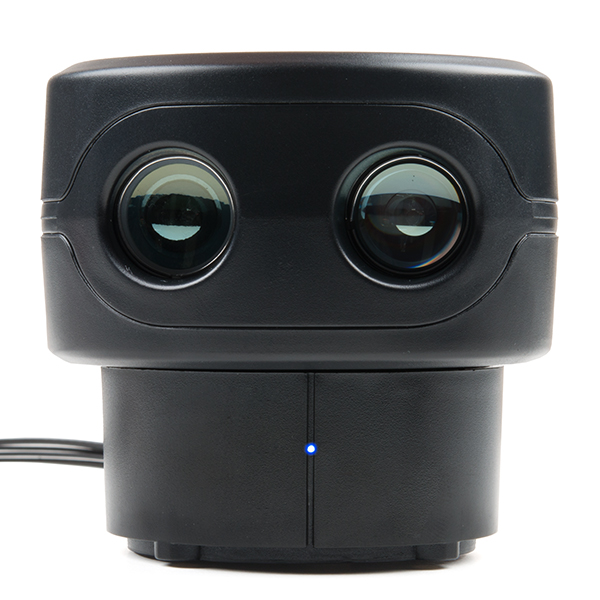
\includegraphics[width=.35\textwidth]{Img/scanse-sweep}}
    \qquad
    \subfloat[Velodyne VLP-16]{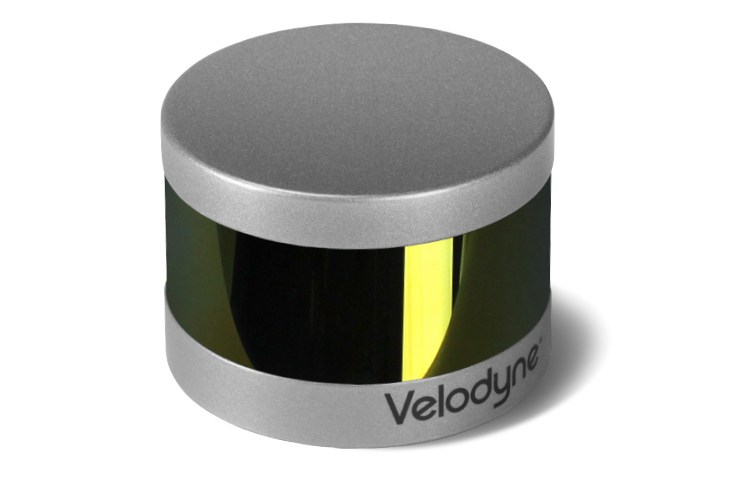
\includegraphics[width=.5\textwidth]{Img/vlp-16}}
    \caption{Algunos LIDAR comerciales}
    \label{fig:lidars}
\end{figure}

\subsubsection{Cámara}
Las cámaras en su versión más simple tienen la característica de ser más económicas y sencillas de montar respecto al resto de los sensores utilizados para el SLAM (tal como el LiDAR), además de no emitir señales al entorno para obtener las características del mismo. A la hora de realizar el SLAM. el modelo de sensado de las cámaras consiste básicamente en un mapeo entre el entorno tridimencional y el plano de la imagen bidimensional. Dependiendo del tipo de cámara (monocular, estéreo, omnidireccional, RGB-D, entre otras), es posible utilizar diferentes modelos matemáticos que permitan relacionar puntos del mundo con su respectiva representación en la imagen.

Para las cámaras monoculares, la línea de base entre las imágenes debe estimarse a partir de la odometría, lo que da lugar al problema de SLAM monocular bien estudiado [124, 125]. Otra forma de realizarlo es mediante la percepción de alto nivel, donde se pueden utilizar señales como el tamaño relativo de un objeto para estimar la escala de la imagen y, por lo tanto, la profundidad [126].

En cambio, para las cámaras RGB-D (\textit{D: Depth} - Profundidad) (Fig. \ref{fig:camaras}.b), uno de los métodos presentados en la literatura para la realización del SLAM a partir de las mismas [ENDERS2012] consiste en primero extraer características visuales de las imágenes de color entrantes. Luego, se comparan estas características con las características de imágenes anteriores. Al evaluar las imágenes de profundidad en las ubicaciones de estos puntos de características, se obtienen un conjunto de correspondencias 3D puntuales entre dos cuadros cualquiera. Basándose en estas correspondencias, se estima la transformación relativa entre los marcos utilizando RANSAC [TRIVEDI2013].

Por otro lado, las técnicas de visión estéreo utilizan dos cámaras con una separación entre las mismas fija y conocida (Fig. \ref{fig:camaras}.a). Las correspondencias de características de la imagen se identifican entre las imágenes mediante la geometría epipolar[REF DE CASTRO] [111], y los rangos se calculan cuando se han medido las disparidades de imagen. Los enfoques pasivos sufren desde muchos modos de falla, desde agujeros de profundidad en áreas de imagen sin características visuales, hasta escenas que crean ambigüedades [123].


\subsubsection{Sensores Inerciales}
El término sensor inercial se usa para denotar la combinación de un acelerómetro de tres ejes y un giroscopio de tres ejes. Los dispositivos que contienen estos sensores se denominan comúnmente unidades de medición inercial (IMU), los cuales en muchos casos incluyen tambien un magnetómetro de tres ejes. Estas unidades sensoriales suelen ser usadas para determinar la orientación y posición de objetos a los cuales se encuentran integrados, permitiendo así la incorporación de los mismos en gran número de aplicaciones [7, 59, 109, 156] [DE KOK2017].

Un giroscopio mide la velocidad angular del sensor, es decir, la velocidad de cambio de la orientación del sensor. En cambio, un acelerómetro mide la fuerza específica externa que actúa sobre el sensor. La fuerza específica consiste tanto en la aceleración del sensor como en la gravedad de la tierra. Estos sensores tienen el inconveniente de presentar un \textit{bias} variable en el tiempo que afecta su funcionamiento. Por otro lado, los magnetómetros son los encargados de medir el campo magnético en el que el objeto se encuentra sumergido, obteniendo así información absoluta del ambiente y no referida únicamente al objeto en si.

Hoy en día, muchos de estos sensores se basan en la tecnología de sistemas microelectromecánicos (MEMS). Los componentes de MEMS son pequeños, ligeros, económicos, tienen un bajo consumo de energía y tiempos de arranque cortos. Su precisión ha aumentado significativamente con los años.

\begin{figure}
    \centering
    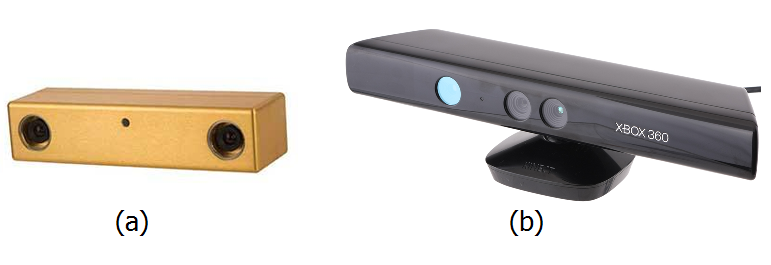
\includegraphics[width=.9\textwidth]{Img/bumblekinect}
    \caption{Cámaras: (a) Bumblebee 2, (b) Kinect}
    \label{fig:camaras}
\end{figure}

\subsubsection{Encoders}
El objetivo de los encoders es medir las rotaciones relativas de la rueda a la que están asociados. Los encoders normalmente se fijan a la salida del motor o de la caja de cambios, con opciones de diseño que a menudo cambian la resolución angular con la máxima velocidad. Los efectos de resolución y muestreo a menudo producen mediciones ruidosas que requieren filtrado digital. La odometría basada en ruedas supone que no hay deslizamiento entre las ruedas y el terreno. En la práctica, los robots móviles con frecuencia superan la fricción estática y rodante, y cuando una o más ruedas giran o se deslizan, pueden ocurrir grandes errores de odometría. La pendiente del terreno, la fricción y otras propiedades pueden variar, incluso entre ruedas individuales. Los robots de accionamiento diferencial con cuatro ruedas a menudo experimentan grandes errores de odometría cuando giran, ya que se requiere un deslizamiento de las ruedas para girar [150].

\subsubsection{GPS}
El GPS es un sistema de navegación georreferenciado basado en satélites mediante los cuales estima la latitud, longitud y altitud del objeto en cuestión. Debido a esto, el mismo tiene su campo de aplicación principalmente en ambientes al aire libre, donde mediante la triangulación entre 4 o más satélites puede determinar la ubicación del objeto en cuestión. Debido a esto y a que, entre otros factores, su principio de funcionamiento se basa en medir el tiempo que tardó la señal disparada por un satélite en ser recibida por el propio sensor, el mismo cuenta con precisiones variables dependiendo de la posición de los satélites [162]. Estos sesgos y errores de grandes pasos hacen que la navegación robótica con GPS sea problemática, especialmente con grandes equipos de robots que operan en entornos urbanos y durante muchas horas. [CARLSON2010]

\subsection{Algoritmos de SLAM}
Los mapas SLAM se construyen a partir de millones de lecturas de sensores, que se comparan entre sí en un paso de asociación de datos que depende completamente de las estimaciones de \textit{pose} actuales. La evaluación y la reevaluación de estas asociaciones de datos, al mismo tiempo que se calcula y actualiza todo el historial de \textit{poses} del robot, describe el problema de \textit{full SLAM} \textbf{[ref 6 de reid2016]}. Si bien este problema no puede resolverse para entornos no triviales, los enfoques descritos en la literatura a menudo producen resultados útiles en entornos del mundo real. En concreto, con el fin de reducir la complejidad del algoritmo se toman como supuestos comunes que el \textit{entorno es estático}, es decir, que el mapa no varía con el tiempo, y por segundo que las taryectorias de los robots \textit{pueden predecirse}, logrando así que los modelos de movimiento puedan predecir dónde es probable que esté un robot, permitiendo que la búsqueda de asociaciones de datos comience cerca del óptimo global.

En esta sección se describen algunos de los enfoques principales que se encuentran en la literatura respecto al tema en cuestión.

\subsubsection{GraphSLAM}

\subsubsection{EKF SLAM}
El filtro de Kalman es uno de los filtros basados en la estimación Bayesiana más conocidos, el cual asume que los modelos matemáticos utilizados son lineales y las distribuciones de sus componentes Gaussianas. En SLAM, sin embargo, los modelos utilizados suelen ser no lineales, por lo que se requiere realizr una linealización apropiada. Mediante el uso de una serie de Taylor alrededor el estado estimado actual, el \textit{Filtro de Kalman Extendido} (EKF) linealiza dicho modelo no lineal.

El enfoque del EKF para solucionar el problema de SLAM es mediante el uso de datos de sensores recopilados a partir del movimiento y la rotación del robot. Esto se puede hacer, por ejemplo, utilizando encoders y una IMU. Además, también es necesario recopilar información del entorno mediante, por ejemplo, el uso de un LIDAR. Con estos datos, el algoritmo realiza un seguimiento del lugar donde probablemente se ubica el robot dentro de un mapa, así como un seguimiento de los puntos de referencia específicos observados.

Al igual que con el filtro de Bayes general, el EKF itera un ciclo de \textit{prediction-update}:

\paragraph{Prediction} Predecir el estado actual expresado por la media predicha y la covarianza predicha. Estos se calculan en función de la entrada de control, las matrices, la covarianza anterior y la media anterior.

\paragraph{Update} La idea detrás del paso de corrección es la asociación de datos el cual, como se dijo anteriormente, tiene el objetivo principal de distinguir entre un hito observado anteriormente y uno recientemente observado. Cuando se produce una nueva medición, en primer lugar se almacenan las ubicaciones de los puntos de referencia recientemente observados. Después de eso, se asocian puntos de referencia observados previamente con los observados recientemente. Además, se calcula la ganancia de corrección, también conocida como la ganancia de Kalman. Básicamente, es un factor de ganancia de corrección necesario para actualizar la media y la covarianza actuales del estado actual. Sin embargo, la media actual y la covarianza no solo dependen de la ganancia de Kalman, sino que también toman en cuenta la media predicha y la covarianza predicha y la medición.

Además de la complejidad cuadrática, este filtro cuando se aplica al problema SLAM tiene como desventaja sustancial \big{[Csorba 1997 DE SU - FAST-SLAM]}
la sensibilidad a fallas que presenta en las asociaciones de datos. Este problema con el EKF se aplica en situaciones en las que se desconocen las asociaciones de datos. El EKF mantiene una única hipótesis de asociación de datos por observación, típicamente elegida usando una heurística de máxima verosimilitud. Si la asociación de datos elegida por esta heurística es incorrecta, el efecto de incorporar esta observación en el EKF nunca se puede eliminar.

\subsubsection{FastSLAM}
